%\documentclass[letterpaper,draft]{beamer}
%\documentclass[letterpaper,handout]{beamer}
\documentclass[letterpaper]{beamer}

%---multiple pages on one sheet, ADD for handout--
%\usepackage{pgfpages}
%\pgfpagesuselayout{4 on 1}[letterpaper, landscape, border shrink=1mm]
%-------------------------------------------------
\usepackage{amsmath,amsfonts}
%\usepackage[misc]{ifsym} % for the dice symbol \Cube{}
%\usepackage{booktabs}
%\usepackage{mdwlist}
\usepackage{amsfonts}
%\usetheme{Copenhagen}
%\usetheme{warsaw}
\setbeamertemplate{navigation symbols}{}
\usepackage[english]{babel}
\def\ul{\underline}
% or whatever

\usepackage[latin1]{inputenc}
\subject{Talks}

\def\Sum{\sum\nolimits}
\def\Prod{\prod\nolimits}
\def\P{\mathbb{P}}
\def\p{\mathrm P}
\def\E{\mathbb E}
\def\V{\mathrm{Var}}
\def\CV{\mathrm{Cov}}
\def\X{\mathcal{X}}
\def\dt{\Delta}
\def\typo#1{\alert{#1}}
%-------------Answers------------
\def\Hide#1#2{\ul{~~~\onslide<#1>{\alert{#2}}~~~}}
\def\hide#1#2{\ul{~~\onslide<#1>{\alert{#2}}~~}}
%------Centered Page Number------
\defbeamertemplate{footline}{centered page number}
{%
  \hspace*{\fill}%
  %\usebeamercolor[fg]{page number in head/foot}%
  %\usebeamerfont{page number in head/foot}%
  \small Lecture \chapnum\ - \insertframenumber%
  \hspace*{\fill}\vskip2pt%
}

%\usepackage{tikz}
%\usebackgroundtemplate{%
%\tikz\node[opacity=0.3] {\includegraphics[height=\paperheight,widht=\paperwidth]{ctanlion}};}

%\usebackgroundtemplate{%
%  %\rule{0pt}{\paperheight}%
%  \parbox[c][\paperheight][c]{\paperwidth}{\centering\includegraphics[width=.65\paperwidth]{UClogo.pdf}}
%  %\hspace*{\paperwidth}
%}

\def\chapnum{22\&23}
%--------------------------------
\setbeamertemplate{footline}[centered page number]

\title{STAT253/317 Winter 2019 Lecture \chapnum} \date{} \author{Yibi Huang}
\begin{document}
% ----------------------------------------------------------------------
\begin{frame}\maketitle
\bigskip
\begin{center}\large
\begin{tabular}{ll}
\multicolumn{2}{l}{Chapter 10  Brownian Motion}\\[5pt]
$\bullet$ & Brownian Motion as a Limit of Random Walk\\
$\bullet$ & Brownian Motion as a Gaussian Process\\
 10.2 & Hitting Time, Maximum Value, Reflection Principle
\end{tabular}
\end{center}
\end{frame}
% ----------------------------------------------------------------------
\begin{frame}{Generalized Random Walk}
The symmetric simple random walk $\{Y_n, n\ge 1\}$ can be defined alternatively as
a sum of i.i.d. random variables
$$
Y_n = X_1+X_2+\cdots+X_n,\quad n\ge 1
$$
where $X_i$'s are i.i.d. with distribution
$$
X_i=\begin{cases}1&\text{w/ prob. }0.5\\-1& \text{w/ prob. }0.5\end{cases}
$$
Generally, for any sequence of i.i.d random variables $X_1,X_2,\ldots$ from an arbitrary distribution with $\E[X_i]=0$, $\V(X_i)=\sigma^2$, the partial sum process
$$
Y_n = X_1+X_2+\cdots+X_n,\quad n\ge 1
$$
is also called a \structure{\bf (generalized) random walk}.
\end{frame}
% ----------------------------------------------------------------------
\begin{frame}{10.1 Brownian Motion as a Limit of Random Walk}
The Browian motion is in fact a limit of rescaled generalized random walk.

Let $X_1,X_2,\ldots$ be i.i.d. random variables, $\E[X_i]=0$, $\V(X_i)=\sigma^2$. Define
$$
X(t)=\dt x(X_1+\ldots+X_{\lfloor t/\dt t\rfloor})
$$
where $\lfloor t/\dt t\rfloor$ is the integer part of $t/\dt t$.\par\smallskip
We'd like to find the limit of $X(t)$ as \underline{$\dt t$ and $\dt x$ both $\to 0$}.

Observe
$$
\E[X(t)]=0 ,\quad
\V(X(t))=\sigma^2(\dt x)^2\left\lfloor \frac{t}{\dt t} \right\rfloor,
$$
To have a non-trivial limit, $\dt t$ and $\dt x$ must maintain the relationship
$$\dt t=c(\dt x)^2.$$
as they approach 0.
Let's take $c=1.$ In this case, as $\dt t\to 0$, $\dt x\to 0$, and $\dt t=(\dt x)^2$, we have
$$
\E[X(t)]=0,\quad\V(X(t))\to\sigma^2t,
$$
\end{frame}
% ----------------------------------------------------------------------
\begin{frame}
Moreover, since $\dt x=\sqrt{\dt t}$, by CLT
$$
X(t)=\dt x(X_1+\ldots+X_{\lfloor \frac{t}{\dt t} \rfloor})\approx\sqrt{t}\sigma\frac{X_1+\ldots+X_{\lfloor \frac{t}{\dt t}\rfloor}}{\sqrt{\lfloor t/\dt t\rfloor}\sigma}\to N(0,\sigma^2t)
$$
in distribution.\par\bigskip

Observe that the discrete-time process $$\{X(t),\;t=n\dt t,\;n=0,1,2\ldots\}$$ has
\structure{\em independent} and \structure{\em stationary increments} since
\begin{align*}
X(s)&= \dt x(X_1+\ldots+X_{\lfloor \frac{s}{\dt t}\rfloor}),\;\text{and }\\[-2pt]
X(t)-X(s)&= \dt x(X_{\lfloor \frac{s}{\dt t}\rfloor+1}+\ldots+X_{\lfloor \frac{t}{\dt t}\rfloor})
\end{align*}
are independent, and for $t=l\dt t > s=m\dt t$, the distribution of $X(t)-X(s)$
depends on the number of terms $\lfloor \frac{t}{\dt t}\rfloor-\lfloor \frac{s}{\dt t}\rfloor$ $=(l-m)=(t-s)/(\dt t)$ in the sum, but not $s$.\medskip

Thus the limit of $X(t)$ is a process with {\bf independent} and {\bf stationary increments}.
\end{frame}
% ----------------------------------------------------------------------
\begin{frame}{Definition of a Brownian Motion}
\textbf{Definition 1}
A stochastic process $\{B(t), t \ge 0\}$ is said to be a Brownian Motion if
\begin{itemize}
\item[(i)] $B(0) = 0$;
\item[(ii)] $\{B(t), t \ge 0\}$ has stationary and independent increments;
\item[(iii)] for every $t,s > 0$, $B(t+s)-B(s)\sim N(0,\sigma^2t)$
\end{itemize}
A Brownian motion with $\sigma=1$ is called a \structure{\em standard Brownian
motion process}

\medskip\hrule\medskip
In fact, we can show that, as a function of $t$, the path of $B(t)$ is \structure{\bf continuous} w/ prob. 1.
\end{frame}
% ----------------------------------------------------------------------
\begin{frame}{Covariance Function of a Brownian Motion}
For $t>s$
\begin{align*}
\CV[B(t),B(s)]&=\CV[B(t)-B(s)+B(s),B(s)]\\
&=\CV[B(t)-B(s),B(s)]+\CV[B(s),B(s)]\\
&=0+\V[B(s)]\quad(\text{by indep. increment})\\
&=\sigma^2s
\end{align*}
The function
$$C(s, t)=\CV(B(t),B(s))=\sigma^2\min(s,t)$$
is called the {\bf covariance function} of the Brownian motion process.\bigskip
\end{frame}
% ----------------------------------------------------------------------
\begin{frame}{10.6 Gaussian Processes}
\textbf{Definition 10.2.}~~
A stochastic process $\{X(t), t\ge 0\}$ is called a \structure{\em Gaussian process} if $X(t_1), \ldots ,X(t_n)$ has a multivariate normal distribution for all $t_1, \ldots , t_n.$\bigskip

Because a multivariate normal distribution is completely determined by the
marginal mean values and the covariance values it follows that the properties of a Gaussian process is completely determined by its \structure{\em mean function} $$m(t)=\E[X(t)]$$ and \structure{\em covariance function} $$C(s,t)=\CV(X(s),X(t)).$$

That is, two Gaussian processes are the same if\medskip

\fboxrule=1pt
\fboxsep=6pt
\fbox{their {\bf mean functions} and {\bf covariance functions} are identical.}
\end{frame}
% ----------------------------------------------------------------------
\begin{frame}{Brownian Motion as a Gaussian Process}
Alternatively, a Brownian motion can be defined as a Gaussian process
with mean function
$$m(t)=\E[B(t)]=0$$ and covariance function
$$C(s,t)=\CV(B(s),B(t))=\sigma^2\min(s,t).$$
\hrule\medskip
\structure{\bf Properties of a Brownian Motion}\par\smallskip

Let $\{B(t), t \ge 0\}$ be a standard Brownian motion.
One can prove each of the following processes below is also a standard Brownian motion
by showing they are all Gaussian processes with the same mean function and covariance function as the standard Brownian motion.
\begin{center}
\begin{tabular}{@{}l@{\;}l@{\qquad}l@{\;}l@{}}
(i) & $\{-B(t), t \ge 0\}$ & (ii) & $\{B(t+s)-B(s), t \ge 0\}$\\
(iii)&  $\{a B(t/a^2), t \ge 0\}$ & (iv)& $\{tB(1/t), t \ge 0\}$
\end{tabular}
\end{center}
\end{frame}
% ----------------------------------------------------------------------
\begin{frame}{Properties of a Brownian Motion (Proofs)}
We'll prove (iv) only. The proofs for the rest are similar.
Clearly $\{tB(1/t), t \ge 0\}$ is a Gaussian process since it is a linear function of a Brownian motion process.
\begin{align*}
\E[tB(1/t)]&=t\E[B(1/t)]=0\quad\text{ since }B(1/t)\sim N(0, 1/t)\\
\CV[tB(1/t),sB(1/s)]&=ts\CV[B(1/t),B(1/s)]\\
&=ts\min\Big(\frac{1}{t},\frac{1}{s}\Big)=\begin{cases}
ts(1/t)=s&\text{if }t>s\\
ts(1/s)=t&\text{if }t\le s
\end{cases}\\
&=\min(s,t)
\end{align*}
As the Gaussian process $\{tB(1/t), t \ge 0\}$ has the same mean function and variance function as a standard Brownian motion, it is also a standard Brownian motion.
\end{frame}
% ----------------------------------------------------------------------
%\begin{frame}%{Joint Distribution of $B(t_1),B(t_2), \ldots , B(t_n)$}
%To derive the joint density of $B(t_1),B(t_2), \ldots , B(t_n),$ %at $B(t_1)=x_1,B(t_2)=x_2,\ldots,B(t_n)=x_n$,
%we may first derive the joint density of
%\begin{align*}
%Y_1&=B(t_1)\sim N(0,\sigma^2t_1),\\
%Y_k&=B(t_k)-B(t_{k-1})\sim N(0,\sigma^2(t_k-t_{k-1}),\ k=2,\ldots,n.
%\end{align*}
%Since $B(t)$ has independent increments, $Y_1,\ldots,Y_n$ are independent. Their joint density is thus
%$$f_{Y_1}(y_1)f_{Y_2}(y_2)\ldots f_{Y_n}(y_n)
%=\prod_{k=1}^n\frac{\exp\left(-\frac{y_k^2}{2(t_k-t_{k-1})}\right)}{\sqrt{2\pi(t_k-t_{k-1})}}$$
%where $t_0=0$. Make a change of variables $B(t_1)=Y_1$, $B(t_k)=Y_1+\ldots+Y_k$, $k=2\ldots,n.$
%Note that the Jacobian is
%$$\det\left(\frac{\partial(y_1,y_2,\ldots,y_n)}{\partial(x_1,x_2,\ldots,x_n)}\right)=1$$
%The joint density of $B(t_1)=x_1,\ldots, B(t_n)=x_n$ is simply
%$$f_{Y_1}(x_1)f_{Y_2}(x_2-x_1)\ldots f_{Y_n}(x_n-x_{n-1})
%=\prod_{k=1}^n\frac{\exp\left(-\frac{(x_k-x_{k-1})^2}{2(t_k-t_{k-1})}\right)}{\sqrt{2\pi(t_k-t_{k-1})}}$$
%\end{frame}
% ----------------------------------------------------------------------
\begin{frame}{Conditional Distribution}
Given $B(t)=x$, what is the conditional distribution of $B(s)$?\bigskip

If $t<s$, since Brownian motion has independent increments,
$B(s)-B(t)$ is independent of $B(t)$, and hence
given $B(t)=x$, the condition distribution of $B(s)-B(t)$ is the same as its unconditional distribution.
\begin{align*}
(B(s)|_{B(t)=x})&=B(t)+[B(s)-B(t)]\\
&=x+\underbrace{B(s)-B(t)}_{\sim N(0,\,\sigma^2(s-t))}\\
&\sim N(x,\,\sigma^2(s-t)).
\end{align*}
\end{frame}
% ----------------------------------------------------------------------
\begin{frame}
What if $s<t$?\bigskip

If we can find a scalar $c$ such that $\CV(B(s)-cB(t),B(t))=0$,
then
$$
B(s)-cB(t)\text{ and $B(t)$ are independent.}
$$
Thus the conditional distribution of of $B(s)-c B(t)$ given $B(t)$ is the same as its unconditional distribution $N(0,\sigma^2(s-2cs+c^2t)).$
Given $B(t)=x,$
\begin{align*}
B(s)&=c\underbrace{B(t)}_{x}+\underbrace{B(s)-cB(t)}_{\sim N(0,\sigma^2(s-2cs+c^2t))}
\sim N\left(cx,\sigma^2(s-2cs+c^2t)\right).
\end{align*}
Because
\begin{align*}
\CV(B(s)-cB(t),B(t))&=\CV(B(s),B(t))-\CV(cB(t),B(t))\\
&=\sigma^2s-c\sigma^2t=\sigma^2(s-ct)
\end{align*}
we know $c=s/t$. Thus the conditional distribution of $B(s)$ given $B(t)=x$ for $s<t$ is
$$ N\left(\frac{sx}{t},\sigma^2\frac{s(t-s)}{t}\right).$$
\end{frame}
% ----------------------------------------------------------------------
%\begin{frame}{Brownian Bridge}
%Let $\{B(t),t\ge 0\}$ be a standard Brownian motion.
%The process $\{B(t), 0\le t\le 1|B(1)=0\}$ is called a \structure{\em Brownian Bridge process}.\bigskip
%
%Properties of a Brownian Bridge process:
%\begin{itemize}
%\item $\E[B(t)|B(1)=0]=0$
%\item $\CV(B(s),B(t)|B(1)=0)=s(1-t)$ \dotfill (HW today)
%\item The process $\{B(t)-tB(1),0\le t\le 1\}$ is also a Brownian bridge process.
% This is an equivalent definition.
%\end{itemize}
%\end{frame}
% ----------------------------------------------------------------------
%\begin{frame}{Application of Brownian Bridge: Kolmogorov-Smirnov Test}
%Suppose $X_1,X_2,\ldots,X_n$ are i.i.d continuous random variables with CDF $F(x)$. An empirical estimate of $F$ is
%$$F_n(s)=\frac{1}{n}\sum_{i=1}^n \mathbf{1}_{\{X_i\le s\}}$$
%Note that for any fixed $s$, $0\le s\le 1$,
%\begin{itemize}
%\item $n F_n(s)\sim Bin(n,F(s))$, and hence $$\V(F_n(s))=F(s)(1-F(s))/n,$$
%\item by SLLN, $F_n(s)\to F(s)$  as $n\to\infty$  with probability 1,
%\item and by CLT, $\sqrt{n}(F_n(s)-F(s))$ is asymptotically normal with mean 0 and variance $F(s)(1-F(s))$
%\end{itemize}
%\end{frame}
%% ----------------------------------------------------------------------
%\begin{frame}
%Moreover, for $s<t$, since
%\begin{align*}
%&\CV(\mathbf{1}_{\{X_i\le \}},\mathbf{1}_{\{X_j\le t\}})=\p(X_i\le s, X_j\le t)-\p(X_i\le s)\p(X_j\le t)\\
%&=\begin{cases}
%\p(X_i\le s)-F(s)F(t)=F(s)(1-F(t))&\text{if }i=j\\
%0 &\text{if }i\neq j
%\end{cases}
%\end{align*}
%we have
%\begin{align*}
%\CV(F_n(s),F_n(t))
%&=\CV\left(\frac{1}{n}\sum_{i=1}^n \mathbf{1}_{\{X_i\le s\}},\frac{1}{n}\sum_{i=1}^n \mathbf{1}_{\{X_i\le %t\}}\right)\\
%&=\frac{1}{n^2}\sum_{i=1}^n \CV(\mathbf{1}_{\{X_i\le s\}},\mathbf{1}_{\{X_i\le t\}})\\
%&=\frac{1}{n^2}\sum_{i=1}^n F(s)(1-F(t))=\frac{1}{n}F(s)(1-F(t))
%\end{align*}
%\end{frame}
%% ----------------------------------------------------------------------
%\begin{frame}
%Hence it is plausible, (and indeed can be proved rigorously) that the limiting process of
%$$\sqrt{n}(F_n(F^{-1}(s))-F(F^{-1}(s)))=\sqrt{n}(F_n(F^{-1}(s))-s)$$
%is a Brownian Bridge, with mean 0 and covariance function given by $s(1-t)$, $0\le s\le t\le 1.$\bigskip
%
%The Kolmogorov-Smirnov statistic for a given CDF $F(x)$ is
%\begin{align*}
%\max_{s}\sqrt{n}(F_n(s)-F(s))&=\max_{0\le s\le 1}\sqrt{n}(F_n(F^{-1}(s))-s)\\
%&\sim \max_{0\le s\le 1}Z(s)
%\end{align*}
%where $\{Z(t),t\ge 0\}$ is the Brownian Bridge process.
%\end{frame}
%% ----------------------------------------------------------------------
\begin{frame}{Hitting Times (First Passage Times)}
Let $T_a=\min\{t: B(t)=a\}$ be the first time the standard Brownian motion process hits {\color{red}$a$}. 
\begin{center}
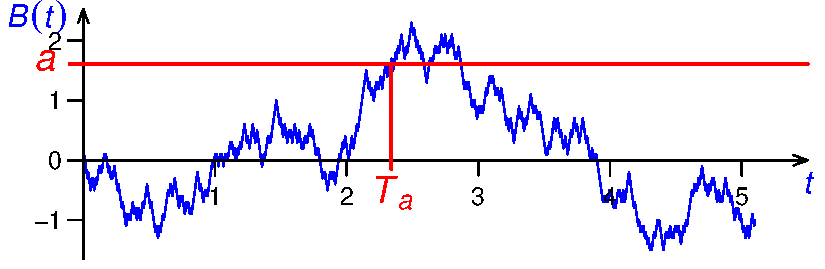
\includegraphics[width=0.9\textwidth]{Lecture22_hitting_time.pdf}
\end{center}
For $a >0$, consider
\begin{align*}
\p(B(t)\ge a) &= \p(B(t)\ge a|T_a \le t)\p(T_a \le t)\\
&\quad+\underbrace{\p(B(t)\ge a|T_a > t)}_{=0}\p(T_a > t)
\end{align*}
The 2nd term on the right is clearly 0, since by continuity,
the process value cannot be $>{\color{red}a}$ without having yet hit {\color{red}$a$}.
\end{frame}
% ----------------------------------------------------------------------
\begin{frame}
For the 1st term, note if $T_a \le t$ , then the process hits {\color{red}$a$} at some point in $[0, t]$ and, by symmetry, it
is just as likely to be above or below {\color{red}$a$} at time $t$. That is
$$\p(B(t)\ge a|T_a \le t)= \frac{1}{2}$$
Thus 
$$\p(T_a \le t)= 2\p(B(t)\ge a)=2-2\Phi(a/\sqrt{t}),$$
where $\Phi(x)=\int_{-\infty}^x\frac{1}{\sqrt{2\pi}}e^{-u^2/2}du$ is the CDF of $N(0,1)$.

By symmetry, $T_{-a}$ and $T_a$ are identically distributed. Hence
$$\p(T_a \le t)= \frac{2}{\sqrt{2\pi}}\int_{|a|/\sqrt{t}}^{\infty}e^{-y^2/2}dy.$$

{\bf HW:} Show that $\p(T_a<\infty)=1$ and $\E[T_a]=\infty$ for $a>0.$

\end{frame}
% ----------------------------------------------------------------------
\begin{frame}{Maximum}
Another random variable of interest is
$$\max_{0\le s\le t}B(s).$$
By the continuity of Brownian motion, we know
$$\max_{0\le s\le t}B(s)\ge a \quad\Leftrightarrow\quad T_a\le t$$
Thus the distribution of for $\max_{0\le s\le t}B(s)$ can be derived via $T_a$. For $a >0$
\begin{align*}
\p\left(\max_{0\le s\le t}B(s) \ge a\right) &= \p(T_a \le t)\\
&= 2\p(B(t)\ge a)=\p(|B(t)|\ge a)\\
&=2-2\Phi(a/\sqrt{t})
\end{align*}
Note this means $\displaystyle{\max_{0\le s\le t}B(s)}$ have the same distribution as $|B(t)|$.
\end{frame}
% ----------------------------------------------------------------------
\begin{frame}{Stopping Time}
For a continuous time stochastic process $\{X(t),t\ge 0\}$,
a \structure{\em stopping time $T$ with respect to} $\{X(t),t\ge 0\}$ is a nonnegative random variable, such that
the event $\{T\le t\}$ depends only on $\{X(s),0\le s\le t\}.$\bigskip

\begin{block}{\bf Example}
The hitting time $T_a=\min\{t: B(t)=a\}$ is a stopping time since
the event $\{T_a\le t\}$ is identical to the event $\Big\{\displaystyle\max_{0\le s\le t}B(s)\ge a\Big\}$
\end{block}
\begin{center}
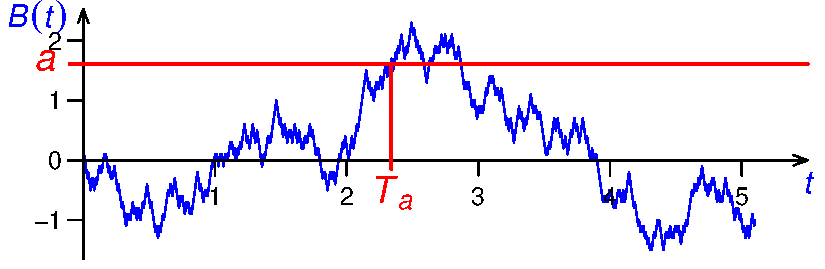
\includegraphics[width=0.9\textwidth]{Lecture22_hitting_time.pdf}
\end{center}

\end{frame}
% ----------------------------------------------------------------------
\begin{frame}{Strong Markov Property}
Let $\{B(t),t\ge 0\}$ be a standard Brownian Motion, and let $T$ be a stopping time respective to $\{B(t),t\ge 0\}$.
Then
\begin{itemize}
\item[(a)] Define $Z(t)=B(t+T)-B(T)$, $t\ge 0$.\\ Then $\{Z(t), t\ge 0\}$ is also a standard Brownian Motion
\item[(b)] For each $t>0$, $\{Z(s), 0\le s\le t\}$ is independent of $\{B(u), 0\le u\le T\}$
\end{itemize}\medskip

\begin{center}
\only<1>{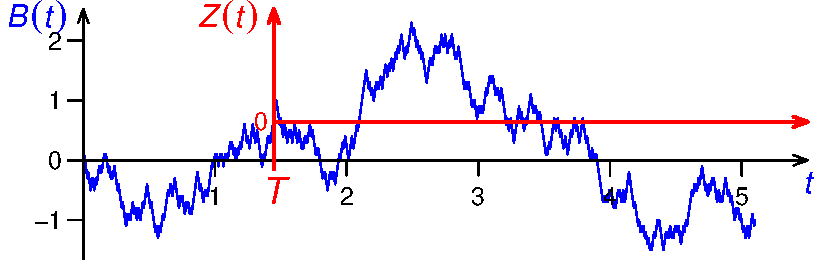
\includegraphics[width=\textwidth]{Lecture22_StrongMarkovProperty1.pdf}}%
\only<2->{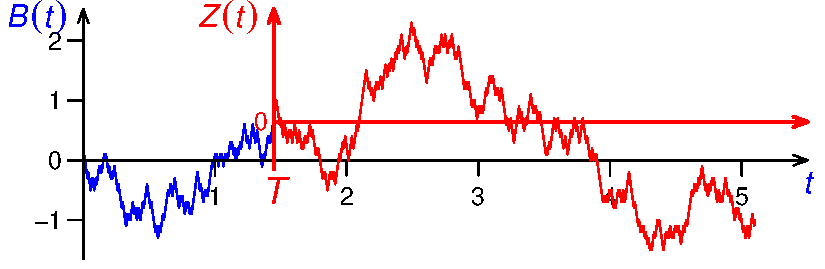
\includegraphics[width=\textwidth]{Lecture22_StrongMarkovProperty2.pdf}}
\end{center}

\end{frame}
% ----------------------------------------------------------------------
\begin{frame}{Reflection Principle}
Let $T_a$ be the first passage time to the value $a$ of a standard Brownian Motion $\{B(t),t\ge 0\}$.
Define a new process
$$
\overline{B}(t)=
\begin{cases}
B(t) &\text{for } t\le T_a\\
2a-B(t) &\text{for } t> T_a
\end{cases}
$$
Then $\{\overline{B}(t),t\ge 0\}$ is also a standard Brownian Motion.

\begin{center}
\only<1>{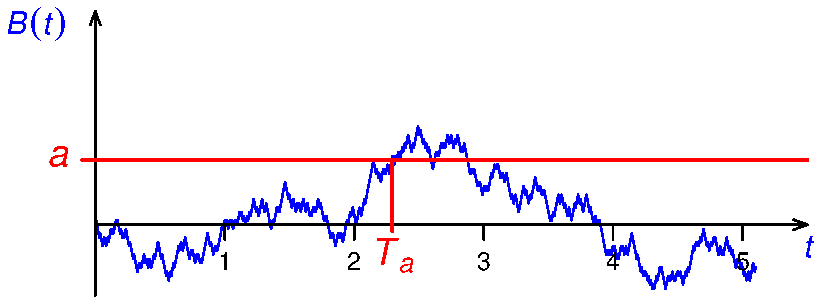
\includegraphics[width=\textwidth]{Lecture22_ReflectionPrinciple1.pdf}}%
\only<2->{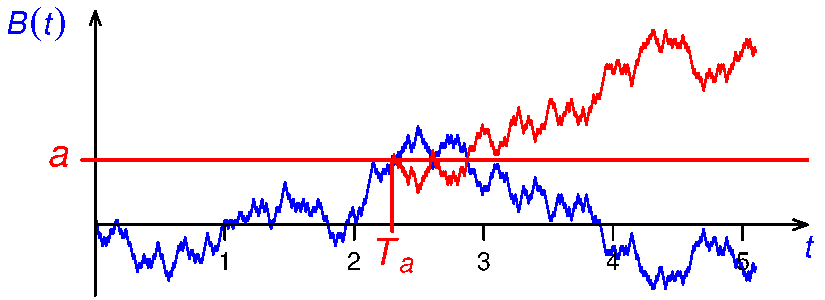
\includegraphics[width=\textwidth]{Lecture22_ReflectionPrinciple2.pdf}}
\end{center}

\end{frame}
% ----------------------------------------------------------------------
\begin{frame}{Proof of the Reflection Principle}
\begin{flushright}
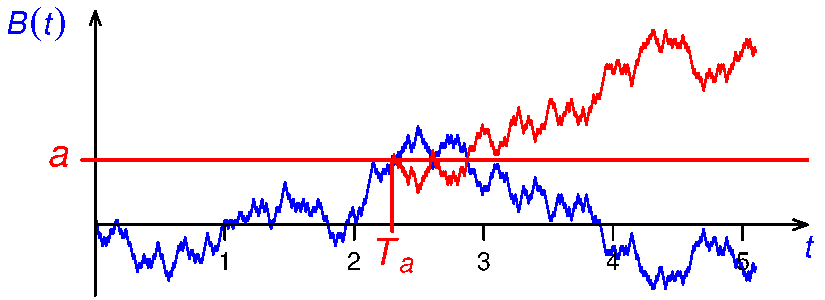
\includegraphics[width=0.75\textwidth]{Lecture22_ReflectionPrinciple2.pdf}
\end{flushright}

\vspace{-16pt}For $t>T_a$, note
$$B(t)=a+B(t)-a=B(T_a)+B(t)-B(T_a).$$\vspace{-12pt}

\begin{itemize}
\item By Strong Markov Property,
$B(s+T_a)-B(T_a)=B(s+T_a)-a$ is also a Brownian Motion, independent of $\{B(s), 0\le s\le T_{a}\}$.
\item Also note that if $\{B(t),t\ge 0\}$ is a standard Brownian motion,
so is $\{-B(t),t\ge 0\}$. Hence $\{a-B(s+T_a),s\ge 0\}$ is also a Brownian Motion.
\end{itemize}
\begin{align*}
\text{So }\{B(t),t>T_a\}&=\{a+B(t)-a,t>T_a\}\\
&\sim \{a+a-B(t),t>T_a\}=\{2a-B(t),t>T_a\}.
\end{align*}
\end{frame}
% ----------------------------------------------------------------------
\begin{frame}{Brownian Motion Absorbed at a Value}
Let $\{B(t)\}$ be a Brownian Motion.\par
For $a> 0$, a Brownian Motion absorbed at a value $a$ is defined as
$$B_a(t)=
\begin{cases}B(t) &\text{if }\max_{0\le s\le t}B(s)< a\\
a & \text{if }\max_{0\le s\le t}B(s)\ge a
\end{cases}$$
What is the distribution of $B_a(t)$? For $x<a$,
\begin{align*}
\p(B_a(t)\le x)&=\p\Big(B(t)\le x,\; \max_{0\le s\le t}B(s)< a\Big)\\[-3pt]
&=\p(B(t)\le x)-\p\Big(B(t)\le x,\; \max_{0\le s\le t}B(s)\ge a\Big)\\[-3pt]
&=\p(B(t)\le x)-\p(B(t)\le x, T_a\le t)
\end{align*}
where the last equality comes from the fact
$$\Big\{\max_{0\le s\le t}B(s)\ge a\Big\}\Leftrightarrow\{T_a\le t\}.$$
\end{frame}
% ----------------------------------------------------------------------
\begin{frame}{Brownian Motion Absorbed at a Value}
\begin{flushright}
\only<1>{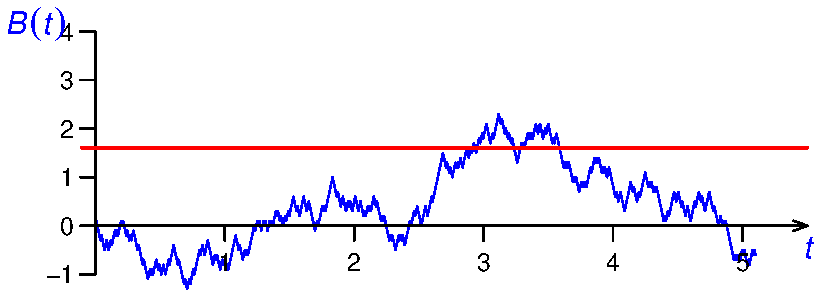
\includegraphics[width=0.65\textwidth]{Lecture22_BM_Absorbed1.pdf}}%
\only<2->{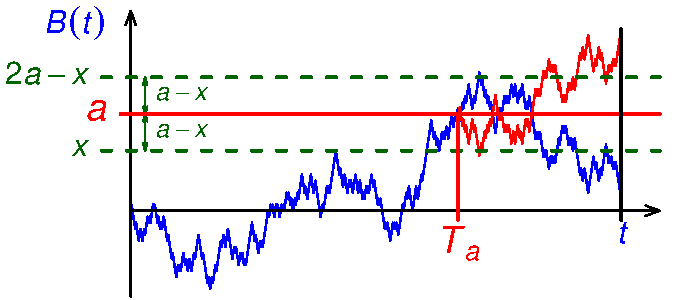
\includegraphics[width=0.65\textwidth]{Lecture22_BM_Absorbed2.pdf}}
\end{flushright}
\vspace{-30pt}By the Reflection principle,
\begin{align*}
&\p(B(t)\le x, T_a\le t)\\
={}&\p(B(t)\ge 2a-x, T_a\le t)=\p(B(t)\ge 2a-x)
\end{align*}
since $x\le a$, $B(t)\ge 2a-x>a$ implies $T_a\le t$.\par\medskip
In summary, the CDF of $B_a(t)$ is\vspace{-5pt}
\begin{align*}
\p(B_a(t)\le x)&=\p\Big(B(t)\le x, \max_{0\le s\le t}B(s)< a\Big)\\
&=\p(B(t)\le x)-\p(B(t)\ge 2a-x)\\
&=\Phi\left(\frac{x}{\sqrt{t}}\right)-1+\Phi\left(\frac{2a-x}{\sqrt{t}}\right)
\end{align*}
\end{frame}
% ----------------------------------------------------------------------
\begin{frame}{More on the Reflection Principle}
Let $\{B(t), t \ge 0\}$ be a standard Brownian motion. Let's try to find the joint distribution of
$$W(t)=\max_{0\le s\le t}B(s) \quad\text{and}\quad  Y(t)=W(t)-B(t)$$
By the Reflection Principle,
%$$\max_{0\le s\le t}B(s)\ge w\;\Leftrightarrow\;T_w\le t,$$
$$
\p(W(t)\ge w,\; B(t)\le x)=\p(T_w\le t,\; B(t)\le x)=\p(B(t)\ge 2w-x)
$$
The joint CDF of $W(t)$ and $B(t)$ is hence,
\begin{align*}
\p(W(t)\le w,\, B(t)\le x)&=\p(B(t)\le x)-\p(W(t)\ge w,\, B(t)\le x)\\
&=\p(B(t)\le x)-\p(B(t)\ge 2w-x)\\
&=\Phi\Big(\frac{x}{\sqrt{t}}\Big)-\left[1-\Phi\Big(\frac{2w-x}{\sqrt{t}}\Big)\right].
\end{align*}
where $\Phi(x)=\int_{-\infty}^x\frac{1}{\sqrt{2\pi}}e^{-u^2/2}du$ is the CDF of $N(0,1)$.
\end{frame}
% ----------------------------------------------------------------------
\begin{frame}
Let $\phi(x)=\dfrac{d}{dx}\Phi(x)=\dfrac{1}{\sqrt{2\pi}}e^{-x^2/2}$ be the density of $N(0,1)$,
Observe that the derivative of $\phi(x)$ is
$$\phi'(x)=\frac{d}{dx}\phi(x)=\frac{-x}{\sqrt{2\pi}}e^{-x^2/2}=-x\phi(x).$$

Take the derivative of the joint CDF of $W(t)$ and $B(t)$ on the previous slide with respect to $w$ and $x$
we get the joint density of $W(t)$ and $B(t)$ below
\begin{align*}
f(w,x)&=\frac{d}{dx}\frac{d}{dw}\left\{\Phi\Big(\frac{x}{\sqrt{t}}\Big)-1+\Phi\Big(\frac{2w-x}{\sqrt{t}}\Big)\Big]\right\}\\
&=\frac{d}{dx}\Big[0+\frac{2}{\sqrt{t}}\phi\Big(\frac{2w-x}{\sqrt{t}}\Big)\Big]\qquad(\text{since }\frac{d}{dw}\left(\Phi\Big(\frac{x}{\sqrt{t}}\Big)-1\right)=0)\\
&=\frac{2w-x}{t}\frac{2}{\sqrt{t}}\phi\Big(\frac{2w-x}{\sqrt{t}}\Big)\qquad(\text{since }\phi'(x)=-x\phi(x))\\
&=\sqrt{\frac{2}{\pi t^3}}(2w-x)\exp\Big(-\frac{(2w-x)^2}{2t}\Big),\; w\ge 0,\; x\le w
\end{align*}
\end{frame}
% ----------------------------------------------------------------------
\begin{frame}
Thus the joint density of $W(t)$ and $B(t)$ is
$$
f(w,x)=\sqrt{\frac{2}{\pi t^3}}(2w-x)\exp\Big(-\frac{(2w-x)^2}{2t}\Big),\; w\ge 0,\; x\le w
$$
By a change of variable of $W(t)$, $Y(t)=W(t)-B(t)$, we can find the desired joint density of $W(t)$, and $Y(t)$
\begin{align*}
g(w,y)&=f(w,w-y)\\
&=\sqrt{\frac{2}{\pi t^3}}(w+y)\exp\Big(-\frac{(w+y)^2}{2t}\Big),\; w\ge 0,\; y\ge 0
\end{align*}
Note that the density is symmetric in $w$ and $y$.\par
Thus $Y(t)$ has the same marginal distribution as $W(t)$, which is also same as $|B(t)|.$
\end{frame}
% ----------------------------------------------------------------------
\end{document}
\begin{frame}{}
\end{frame}
% ----------------------------------------------------------------------
\begin{frame}
\end{frame}
% ----------------------------------------------------------------------
